% 图 77.3 —— 由 `checks/emit_hand.py` 自动拼出（probe 精测 + prims2 图元分解）
%%
% ⚠ 这是**稿子不是成品**：跑 `checks/checkhand.py 77.3` 看指标 + 看叠合图。
%%
%% ⚠ 待核：
%   · 本图 probe 报出阴影族 2 个 —— **本脚本不生成阴影**（要照原书手写）；prims2 的 strokes 里可能含阴影线，核对时留意别画重
%   · 可疑字形 1 项（空心圈 ⊙ 常被认成字母 o）—— 见文件末
%%
\documentclass[12pt]{standalone}
\usepackage{fontspec}
\setsansfont{Arial}
\newfontfamily\mfallback{DejaVu Sans}
\usepackage{tikz}
\begin{document}
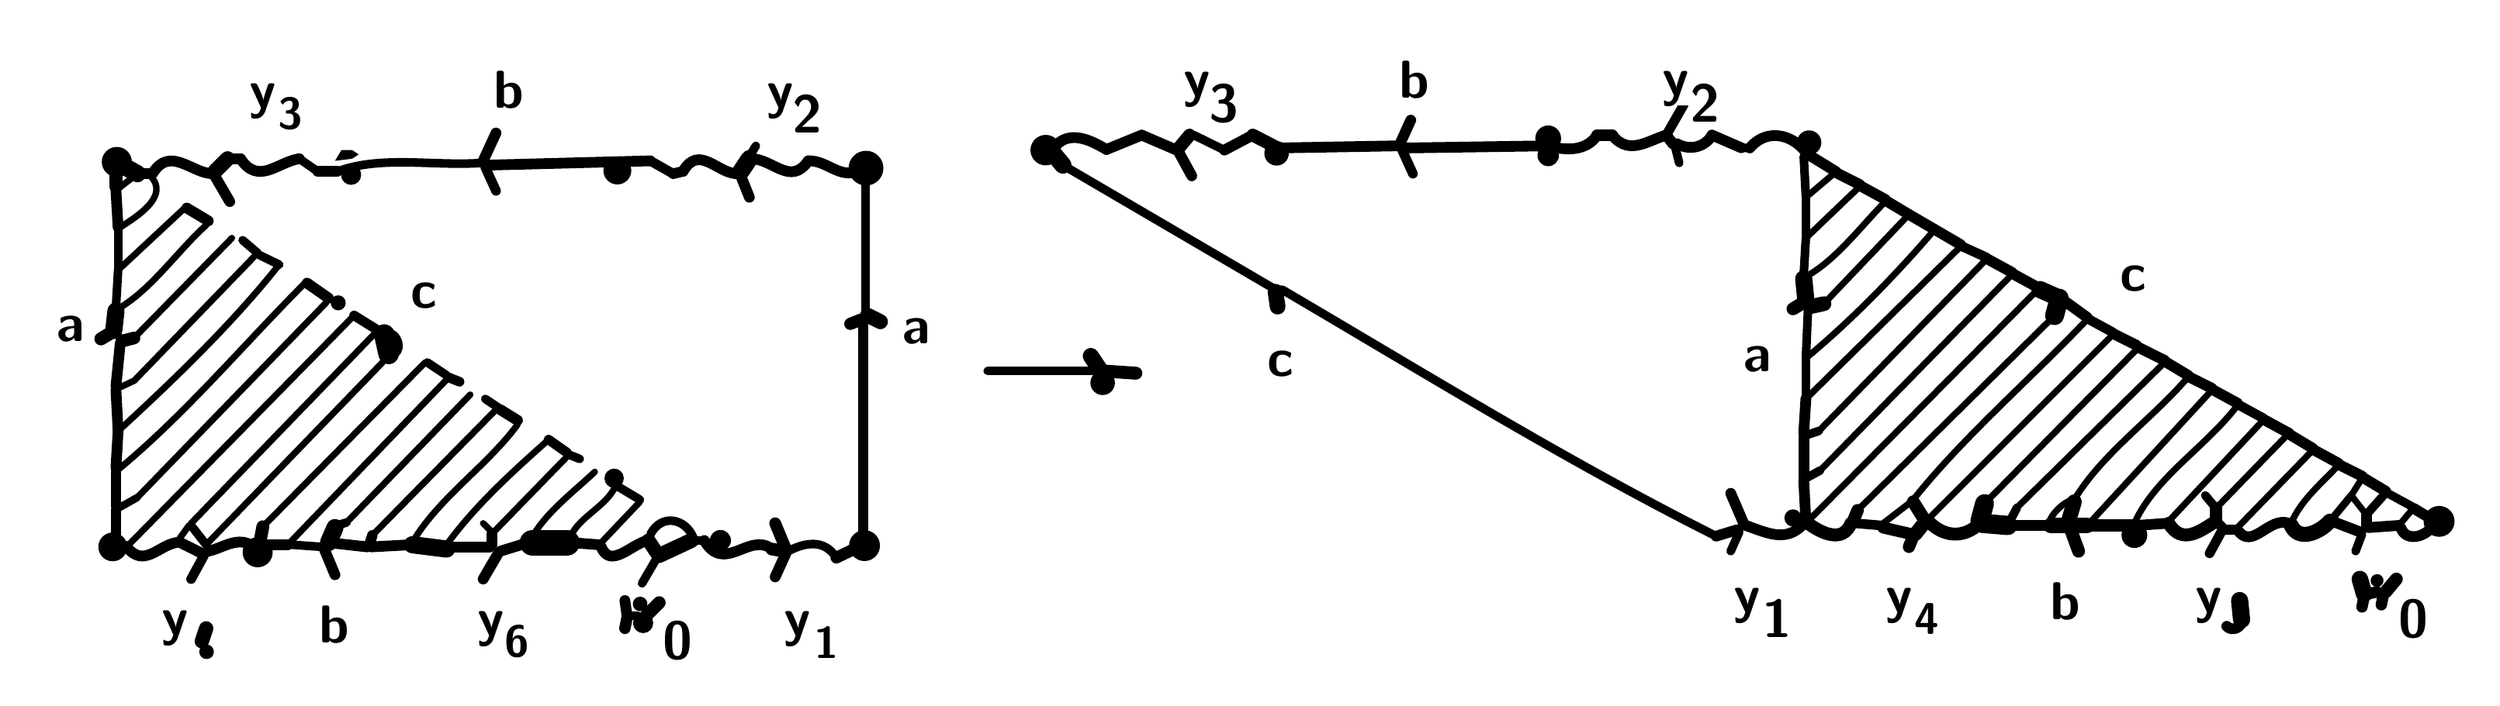
\begin{tikzpicture}[x=1pt, y=-1pt, line width=4.0pt, line cap=round, line join=round]

  %% ════ 填充区（prims2 的 fills）════
  \fill (146.0,65.0) -- (154.0,64.0) -- (157.0,62.0) -- (154.0,60.0) -- (149.0,60.0) -- cycle;

  %% ════ 直线段（prims2 的 strokes）════
  \draw[line width=4.0pt] (288.0,223.0) -- (278.0,217.0);
  \draw[line width=5.0pt] (215.0,260.0) -- (222.0,248.0);
  \draw[line width=7.0pt] (945.0,235.0) -- (952.0,235.0);
  \draw[line width=4.0pt] (296.0,250.0) -- (289.0,262.0);
  \draw[line width=3.0pt] (939.0,125.0) -- (832.0,233.0);
  \draw[line width=4.0pt] (45.0,116.0) -- (44.0,133.0);
  \draw[line width=12.0pt] (238.0,243.0) -- (254.0,243.0);
  \draw[line width=5.0pt] (256.0,243.0) -- (269.0,244.0);
  \draw[line width=5.0pt] (642.0,57.0) -- (647.0,46.0);
  \draw[line width=5.0pt] (1124.0,233.0) -- (1114.0,227.0);
  \draw[line width=8.0pt] (1033.0,270.0) -- (1033.9,278.9);
  \draw[line width=4.0pt] (831.0,193.0) -- (837.1,190.9);
  \draw[line width=3.0pt] (837.1,190.9) -- (914.0,112.0);
  \draw[line width=5.0pt] (133.0,122.0) -- (143.0,129.0);
  \draw[line width=3.0pt] (45.0,78.0) -- (54.0,71.0);
  \draw[line width=4.0pt] (546.0,53.0) -- (560.2,60.0);
  \draw[line width=5.0pt] (560.2,60.0) -- (573.4,53.0);
  \draw[line width=6.0pt] (573.4,53.0) -- (585.0,59.0);
  \draw[line width=5.0pt] (585.0,59.0) -- (641.0,58.0);
  \draw[line width=4.0pt] (86.0,244.0) -- (79.0,235.0);
  \draw[line width=3.0pt] (86.0,244.0) -- (171.0,156.0);
  \draw[line width=5.0pt] (141.0,246.0) -- (146.0,258.0);
  \draw[line width=6.7pt] (84.0,289.0) -- (86.0,283.0);
  \draw[line width=5.0pt] (975.0,146.0) -- (985.0,151.0);
  \draw[line width=3.0pt] (902.0,106.0) -- (832.0,175.0);
  \draw[line width=8.0pt] (44.0,135.0) -- (43.0,144.0);
  \draw[line width=4.5pt] (245.5,195.0) -- (254.0,201.0);
  \draw[line width=5.0pt] (845.0,70.0) -- (832.0,62.0);
  \draw[line width=6.5pt] (292.0,242.0) -- (296.0,248.0);
  \draw[line width=3.0pt] (1055.0,193.0) -- (1022.0,227.0);
  \draw[line width=5.0pt] (199.0,245.0) -- (218.0,245.0);
  \draw[line width=7.0pt] (953.0,234.0) -- (956.0,224.0);
  \draw[line width=9.6pt] (171.0,155.0) -- (169.0,146.0);
  \draw[line width=3.0pt] (125.0,243.0) -- (198.0,167.0);
  \draw[line width=5.7pt] (391.0,139.0) -- (386.0,141.0);
  \draw[line width=5.0pt] (830.0,192.0) -- (831.0,176.0);
  \draw[line width=5.5pt] (379.5,250.0) -- (392.0,244.0);
  \draw[line width=7.5pt] (498.0,156.0) -- (502.0,162.0);
  \draw[line width=3.0pt] (880.0,224.0) -- (867.0,234.0);
  \draw[line width=5.0pt] (392.0,140.0) -- (392.0,243.0);
  \draw[line width=6.0pt] (825.0,134.0) -- (830.0,131.0);
  \draw[line width=5.0pt] (857.0,77.0) -- (868.0,83.0);
  \draw[line width=5.0pt] (962.0,138.0) -- (951.0,130.0);
  \draw[line width=5.0pt] (97.0,84.0) -- (90.0,72.0);
  \draw[line width=4.0pt] (260.0,204.0) -- (255.0,202.0);
  \draw[line width=6.0pt] (44.0,67.0) -- (44.0,77.0);
  \draw[line width=6.0pt] (111.0,243.0) -- (112.4,235.6);
  \draw[line width=3.0pt] (112.4,235.6) -- (188.0,159.0);
  \draw[line width=4.0pt] (216.0,176.0) -- (222.0,180.0);
  \draw[line width=4.0pt] (831.0,157.0) -- (832.0,134.0);
  \draw[line width=4.0pt] (831.0,157.0) -- (831.0,175.0);
  \draw[line width=6.5pt] (882.0,239.0) -- (886.0,234.0);
  \draw[line width=5.0pt] (787.3,53.0) -- (800.9,58.9);
  \draw[line width=4.0pt] (800.9,58.9) -- (804.9,59.0);
  \draw[line width=3.0pt] (888.0,232.0) -- (973.0,147.0);
  \draw[line width=5.8pt] (853.0,233.0) -- (855.1,227.9);
  \draw[line width=3.0pt] (855.1,227.9) -- (946.8,137.2);
  \draw[line width=8.8pt] (946.8,137.2) -- (949.0,129.0);
  \draw[line width=5.5pt] (867.0,236.0) -- (880.0,239.0);
  \draw[line width=5.0pt] (830.0,214.0) -- (831.0,233.0);
  \draw[line width=5.3pt] (44.0,244.0) -- (49.0,245.0);
  \draw[line width=5.0pt] (46.0,150.0) -- (44.0,170.0);
  \draw[line width=4.0pt] (501.0,163.0) -- (450.0,163.0);
  \draw[line width=5.0pt] (1089.0,238.0) -- (1076.0,233.0);
  \draw[line width=7.7pt] (1089.0,260.0) -- (1091.0,267.0);
  \draw[line width=8.0pt] (480.0,61.0) -- (485.0,67.0);
  \draw[line width=4.0pt] (485.0,67.0) -- (584.0,125.0);
  \draw[line width=5.0pt] (869.0,84.0) -- (879.0,90.0);
  \draw[line width=4.5pt] (866.0,235.0) -- (854.0,234.0);
  \draw[line width=5.0pt] (74.0,243.0) -- (84.0,248.0);
  \draw[line width=3.0pt] (49.0,245.0) -- (154.9,137.1);
  \draw[line width=4.5pt] (154.9,137.1) -- (166.0,144.0);
  \draw[line width=8.0pt] (831.0,130.0) -- (830.0,120.0);
  \draw[line width=3.0pt] (46.0,115.0) -- (76.0,87.0);
  \draw[line width=5.3pt] (1092.0,267.0) -- (1097.0,266.0);
  \draw[line width=5.0pt] (161.0,245.0) -- (143.0,243.0);
  \draw[line width=7.3pt] (585.0,133.0) -- (584.0,126.0);
  \draw[line width=4.0pt] (103.0,102.0) -- (110.0,108.0);
  \draw[line width=5.0pt] (879.0,90.0) -- (891.0,97.0);
  \draw[line width=3.0pt] (879.0,90.0) -- (839.4,131.6);
  \draw[line width=6.9pt] (839.4,131.6) -- (833.0,133.0);
  \draw[line width=4.0pt] (111.0,109.0) -- (120.0,113.4);
  \draw[line width=6.1pt] (42.0,145.0) -- (37.0,148.0);
  \draw[line width=8.0pt] (182.0,244.0) -- (198.0,246.0);
  \draw[line width=5.9pt] (355.0,247.0) -- (349.4,246.0);
  \draw[line width=4.0pt] (318.0,242.0) -- (314.0,242.0);
  \draw[line width=5.0pt] (799.0,237.0) -- (789.2,240.0);
  \draw[line width=3.0pt] (45.0,171.0) -- (52.5,167.5);
  \draw[line width=3.0pt] (52.5,167.5) -- (109.0,109.0);
  \draw[line width=4.0pt] (800.0,238.0) -- (796.0,247.0);
  \draw[line width=5.0pt] (903.0,104.0) -- (891.0,97.0);
  \draw[line width=5.0pt] (44.0,228.0) -- (44.0,243.0);
  \draw[line width=8.0pt] (146.0,236.0) -- (143.0,243.0);
  \draw[line width=4.5pt] (904.0,105.0) -- (915.0,110.0);
  \draw[line width=5.0pt] (644.0,59.0) -- (711.0,58.0);
  \draw[line width=5.3pt] (281.0,283.0) -- (282.0,278.0);
  \draw[line width=5.0pt] (77.0,87.0) -- (87.0,93.0);
  \draw[line width=5.0pt] (1107.0,235.0) -- (1093.0,236.0);
  \draw[line width=5.0pt] (999.0,234.0) -- (985.0,235.0);
  \draw[line width=5.0pt] (335.0,72.0) -- (339.0,82.0);
  \draw[line width=4.5pt] (199.0,166.0) -- (204.0,168.0);
  \draw[line width=3.0pt] (1113.0,228.0) -- (1108.0,234.0);
  \draw[line width=3.0pt] (78.0,235.0) -- (73.0,242.0);
  \draw[line width=3.0pt] (288.0,224.0) -- (270.0,243.0);
  \draw[line width=4.0pt] (772.0,66.0) -- (770.0,58.0);
  \draw[line width=3.0pt] (219.0,238.0) -- (215.0,234.0);
  \draw[line width=4.0pt] (1090.0,239.0) -- (1087.0,247.0);
  \draw[line width=4.9pt] (308.1,69.9) -- (303.5,71.0);
  \draw[line width=4.5pt] (303.5,71.0) -- (292.9,65.0);
  \draw[line width=5.0pt] (292.9,65.0) -- (217.0,67.0);
  \draw[line width=5.0pt] (1031.0,237.0) -- (1026.0,237.0);
  \draw[line width=4.0pt] (339.0,63.0) -- (342.0,58.0);
  \draw[line width=5.0pt] (846.0,71.0) -- (856.0,76.0);
  \draw[line width=5.0pt] (545.0,72.0) -- (539.0,61.0);
  \draw[line width=5.0pt] (223.0,181.0) -- (231.0,186.0);
  \draw[line width=3.8pt] (46.0,148.0) -- (44.0,145.0);
  \draw[line width=5.5pt] (351.0,234.0) -- (356.0,246.0);
  \draw[line width=7.0pt] (90.0,70.0) -- (96.0,64.0);
  \draw[line width=4.0pt] (126.0,244.0) -- (140.0,245.0);
  \draw[line width=7.0pt] (962.0,235.0) -- (955.0,235.0);
  \draw[line width=4.7pt] (1025.0,236.0) -- (1022.0,233.0);
  \draw[line width=5.0pt] (147.0,70.0) -- (138.0,70.0);
  \draw[line width=4.0pt] (138.0,70.0) -- (129.4,64.0);
  \draw[line width=5.0pt] (102.0,64.0) -- (97.0,64.0);
  \draw[line width=4.5pt] (79.0,260.0) -- (85.0,249.0);
  \draw[line width=5.0pt] (998.0,158.0) -- (986.0,152.0);
  \draw[line width=8.8pt] (912.0,233.0) -- (914.2,224.8);
  \draw[line width=3.0pt] (914.2,224.8) -- (985.0,153.0);
  \draw[line width=3.0pt] (1043.0,187.0) -- (1000.0,233.0);
  \draw[line width=5.0pt] (1092.0,235.0) -- (1092.0,230.0);
  \draw[line width=8.0pt] (949.0,129.0) -- (940.0,125.0);
  \draw[line width=5.0pt] (112.0,244.0) -- (124.0,244.0);
  \draw[line width=5.0pt] (59.0,71.0) -- (54.0,71.0);
  \draw[line width=5.0pt] (830.0,212.0) -- (830.0,194.0);
  \draw[line width=5.0pt] (356.0,248.0) -- (351.0,259.0);
  \draw[line width=4.0pt] (831.0,101.0) -- (831.0,82.0);
  \draw[line width=3.0pt] (831.0,101.0) -- (855.0,78.0);
  \draw[line width=4.0pt] (831.0,101.0) -- (830.0,118.0);
  \draw[line width=4.0pt] (925.0,235.0) -- (929.3,226.7);
  \draw[line width=3.0pt] (929.3,226.7) -- (997.0,160.0);
  \draw[line width=9.0pt] (925.0,235.0) -- (913.0,234.0);
  \draw[line width=5.0pt] (925.0,235.0) -- (943.0,235.0);
  \draw[line width=3.5pt] (45.0,227.0) -- (53.9,222.0);
  \draw[line width=3.0pt] (53.9,222.0) -- (142.0,131.0);
  \draw[line width=8.0pt] (54.0,71.0) -- (45.0,66.0);
  \draw[line width=5.0pt] (1021.0,172.0) -- (1032.0,178.0);
  \draw[line width=5.0pt] (236.0,243.0) -- (223.0,247.0);
  \draw[line width=7.0pt] (400.0,140.0) -- (394.0,137.0);
  \draw[line width=6.0pt] (519.0,164.0) -- (504.0,163.0);
  \draw[line width=5.0pt] (219.0,244.0) -- (219.0,239.0);
  \draw[line width=5.0pt] (538.0,60.0) -- (521.7,53.0);
  \draw[line width=5.0pt] (521.7,53.0) -- (505.3,59.7);
  \draw[line width=5.0pt] (1090.0,212.0) -- (1080.0,207.0);
  \draw[line width=4.0pt] (831.0,82.0) -- (830.0,63.0);
  \draw[line width=3.0pt] (831.0,82.0) -- (844.0,71.0);
  \draw[line width=6.0pt] (544.0,53.0) -- (539.0,59.0);
  \draw[line width=5.0pt] (44.0,79.0) -- (45.0,96.0);
  \draw[line width=4.0pt] (147.0,235.0) -- (151.4,233.6);
  \draw[line width=3.0pt] (151.4,233.6) -- (209.0,174.0);
  \draw[line width=5.0pt] (796.0,220.0) -- (802.0,234.0);
  \draw[line width=4.0pt] (1017.0,221.0) -- (1022.0,227.0);
  \draw[line width=5.3pt] (1099.0,272.0) -- (1100.0,267.0);
  \draw[line width=6.0pt] (1106.0,260.0) -- (1101.0,266.0);
  \draw[line width=3.0pt] (1066.0,201.0) -- (1032.0,236.0);
  \draw[line width=4.0pt] (393.0,136.0) -- (393.0,69.0);
  \draw[line width=5.0pt] (1101.0,219.0) -- (1091.0,213.0);
  \draw[line width=7.0pt] (297.0,249.0) -- (312.0,242.0);
  \draw[line width=5.0pt] (45.0,191.0) -- (44.0,172.0);
  \draw[line width=5.0pt] (45.0,191.0) -- (44.0,208.0);
  \draw[line width=4.5pt] (1044.0,185.0) -- (1033.0,179.0);
  \draw[line width=5.0pt] (1057.0,193.0) -- (1067.0,199.0);
  \draw[line width=5.0pt] (1045.0,186.0) -- (1056.0,192.0);
  \draw[line width=5.0pt] (44.0,226.0) -- (44.0,210.0);
  \draw[line width=5.0pt] (1020.0,171.0) -- (1010.0,166.0);
  \draw[line width=5.1pt] (769.0,57.0) -- (766.0,53.0);
  \draw[line width=4.0pt] (45.0,115.0) -- (45.0,97.0);
  \draw[line width=5.7pt] (881.0,240.0) -- (879.0,245.0);
  \draw[line width=6.0pt] (886.0,232.0) -- (881.0,224.0);
  \draw[line width=4.5pt] (216.0,68.0) -- (221.0,79.0);
  \draw[line width=4.0pt] (1113.0,226.0) -- (1102.0,220.0);
  \draw[line width=5.3pt] (1091.0,268.0) -- (1090.0,273.0);
  \draw[line width=5.5pt] (733.8,53.0) -- (740.8,53.0);
  \draw[line width=3.0pt] (1092.0,230.0) -- (1085.0,221.0);
  \draw[line width=4.0pt] (1092.0,230.0) -- (1100.0,221.0);
  \draw[line width=5.0pt] (181.0,244.0) -- (163.0,245.0);
  \draw[line width=5.0pt] (939.0,124.0) -- (928.0,118.0);
  \draw[line width=6.0pt] (1022.0,227.0) -- (1022.0,233.0);
  \draw[line width=5.0pt] (215.0,65.0) -- (221.0,52.0);
  \draw[line width=5.9pt] (47.0,149.0) -- (52.4,147.6);
  \draw[line width=3.0pt] (52.4,147.6) -- (98.0,101.0);
  \draw[line width=5.0pt] (927.0,117.0) -- (916.0,111.0);
  \draw[line width=6.0pt] (954.0,236.0) -- (958.0,247.0);
  \draw[line width=6.0pt] (297.0,271.0) -- (291.0,277.0);
  \draw[line width=5.0pt] (1079.0,206.0) -- (1068.0,200.0);
  \draw[line width=4.5pt] (766.0,53.0) -- (774.0,39.0);
  \draw[line width=8.0pt] (339.0,64.0) -- (335.0,70.0);
  \draw[line width=4.5pt] (643.0,60.0) -- (648.0,71.0);
  \draw[line width=4.0pt] (831.0,213.0) -- (837.6,209.4);
  \draw[line width=3.0pt] (837.6,209.4) -- (926.0,119.0);
  \draw[line width=4.9pt] (162.0,244.0) -- (163.4,239.6);
  \draw[line width=3.0pt] (163.4,239.6) -- (221.0,181.0);
  \draw[line width=5.0pt] (999.0,159.0) -- (1009.0,165.0);
  \draw[line width=4.5pt] (974.0,145.0) -- (963.0,139.0);
  \draw[line width=3.0pt] (165.0,145.0) -- (79.0,234.0);
  \draw[line width=5.0pt] (281.0,270.0) -- (282.0,277.0);
  \draw[line width=4.5pt] (1025.0,237.0) -- (1019.0,248.0);
  \draw[line width=3.0pt] (254.0,203.0) -- (220.0,238.0);
  \draw[line width=4.0pt] (189.0,159.0) -- (198.0,165.0);
  \draw[line width=3.5pt] (1076.0,232.0) -- (1085.0,221.0);
  \draw[line width=6.0pt] (983.0,235.0) -- (964.0,235.0);
  \draw[line width=3.0pt] (1085.0,221.0) -- (1090.0,213.0);
  \draw[line width=4.0pt] (283.0,277.0) -- (287.0,277.0);
  \draw[line width=3.0pt] (1020.0,172.0) -- (963.0,234.0);

  %% ════ 曲线（prims2 的 curves —— 三段式，坐标同为 (y,x)）════
  \draw[line width=7.0pt] (1057.0,235.0) .. controls (1060.7,242.9) and (1070.7,238.0) .. (1075.0,233.0);
  \draw[line width=5.0pt] (1124.0,233.0) .. controls (1122.0,239.6) and (1110.8,243.8) .. (1108.0,236.0);
  \draw[line width=5.0pt] (1033.9,278.9) .. controls (1034.4,282.5) and (1029.5,284.7) .. (1027.0,282.0);
  \draw[line width=6.0pt] (832.0,234.0) .. controls (837.7,238.3) and (848.2,243.7) .. (852.0,234.0);
  \draw[line width=3.0pt] (198.0,244.0) .. controls (211.1,225.9) and (228.6,210.0) .. (245.5,195.0);
  \draw[line width=3.0pt] (944.0,234.0) .. controls (945.6,229.4) and (950.4,224.6) .. (955.0,223.0);
  \draw[line width=5.0pt] (292.0,242.0) .. controls (285.1,242.7) and (274.3,255.9) .. (270.0,245.0);
  \draw[line width=5.0pt] (1056.0,234.0) .. controls (1046.6,230.6) and (1038.7,247.1) .. (1032.0,237.0);
  \draw[line width=4.0pt] (357.0,247.0) .. controls (364.8,243.0) and (373.7,241.1) .. (379.5,250.0);
  \draw[line width=4.0pt] (313.0,241.0) .. controls (309.6,231.9) and (298.2,229.1) .. (293.0,239.0);
  \draw[line width=3.0pt] (831.0,157.0) .. controls (852.2,139.5) and (873.5,117.5) .. (891.0,97.0);
  \draw[line width=5.0pt] (87.0,247.0) .. controls (93.6,245.7) and (101.2,239.4) .. (108.0,245.0);
  \draw[line width=5.0pt] (771.0,57.0) .. controls (776.7,60.3) and (783.9,58.8) .. (787.3,53.0);
  \draw[line width=5.0pt] (804.9,59.0) .. controls (812.6,49.7) and (824.6,52.5) .. (831.0,61.0);
  \draw[line width=3.0pt] (255.0,242.0) .. controls (258.2,231.8) and (270.6,227.4) .. (276.0,218.0);
  \draw[line width=3.0pt] (831.0,119.0) .. controls (844.7,111.4) and (855.9,96.5) .. (867.0,85.0);
  \draw[line width=5.0pt] (49.0,245.0) .. controls (56.9,255.0) and (63.8,244.4) .. (72.0,243.0);
  \draw[line width=3.0pt] (120.0,113.4) .. controls (98.2,140.9) and (71.3,166.8) .. (45.0,191.0);
  \draw[line width=5.0pt] (349.4,246.0) .. controls (339.2,237.8) and (327.2,257.9) .. (318.0,242.0);
  \draw[line width=4.0pt] (789.2,240.0) .. controls (720.0,205.2) and (653.9,164.3) .. (587.0,125.0);
  \draw[line width=3.0pt] (86.0,95.0) .. controls (72.3,107.4) and (60.8,124.7) .. (45.0,134.0);
  \draw[line width=3.0pt] (46.0,96.0) .. controls (53.4,91.1) and (69.4,81.5) .. (60.0,72.0);
  \draw[line width=5.0pt] (340.0,64.0) .. controls (350.0,64.2) and (358.2,76.9) .. (366.4,65.0);
  \draw[line width=5.0pt] (366.4,65.0) .. controls (375.9,64.6) and (382.5,75.5) .. (392.0,68.0);
  \draw[line width=3.0pt] (881.0,223.0) .. controls (903.7,194.4) and (935.0,167.3) .. (961.0,140.0);
  \draw[line width=5.0pt] (334.0,71.0) .. controls (324.5,71.6) and (315.7,56.8) .. (308.1,69.9);
  \draw[line width=3.0pt] (231.0,188.0) .. controls (217.0,207.1) and (194.0,222.4) .. (182.0,243.0);
  \draw[line width=4.0pt] (214.0,66.0) .. controls (191.2,67.5) and (167.5,62.4) .. (147.0,70.0);
  \draw[line width=5.0pt] (129.4,64.0) .. controls (119.3,65.5) and (110.4,76.6) .. (102.0,64.0);
  \draw[line width=3.0pt] (132.0,122.0) .. controls (103.4,150.7) and (76.6,182.8) .. (45.0,209.0);
  \draw[line width=3.0pt] (984.0,234.0) .. controls (993.5,212.6) and (1017.4,198.3) .. (1032.0,179.0);
  \draw[line width=3.0pt] (956.0,223.0) .. controls (968.8,201.8) and (991.0,186.3) .. (1008.0,167.0);
  \draw[line width=5.0pt] (505.3,59.7) .. controls (497.6,55.2) and (486.9,49.7) .. (480.0,60.0);
  \draw[line width=5.0pt] (830.0,234.0) .. controls (822.1,243.6) and (811.9,238.0) .. (803.0,235.0);
  \draw[line width=6.0pt] (888.0,233.0) .. controls (894.9,240.4) and (904.5,241.3) .. (912.0,234.0);
  \draw[line width=3.0pt] (1078.0,208.0) .. controls (1070.1,216.2) and (1061.1,224.0) .. (1057.0,234.0);
  \draw[line width=5.0pt] (172.0,146.0) .. controls (175.6,147.7) and (176.6,154.4) .. (172.0,155.0);
  \draw[line width=5.0pt] (711.0,58.0) .. controls (719.1,60.3) and (728.8,60.6) .. (733.8,53.0);
  \draw[line width=5.0pt] (740.8,53.0) .. controls (748.6,62.7) and (757.2,55.6) .. (766.0,53.0);
  \draw[line width=3.0pt] (267.0,210.0) .. controls (257.0,219.5) and (243.2,229.7) .. (237.0,242.0);
  \draw[line width=5.0pt] (89.0,71.0) .. controls (79.2,70.8) and (69.1,57.7) .. (61.0,71.0);
  \draw[line width=6.0pt] (1000.0,234.0) .. controls (1006.2,244.5) and (1015.0,237.3) .. (1022.0,233.0);

  %% ════ 实心点 ════
  \fill (477.0,60.0) circle (7.1);
  \fill (711.0,54.5) circle (6.0);
  \fill (832.5,56.5) circle (5.7);
  \fill (44.4,65.5) circle (7.0);
  \fill (393.3,68.4) circle (8.1);
  \fill (584.5,61.5) circle (5.7);
  \fill (711.0,62.5) circle (5.0);
  \fill (277.5,69.5) circle (6.5);
  \fill (153.5,71.5) circle (4.7);
  \fill (147.5,131.2) circle (3.5);
  \fill (503.5,168.5) circle (5.7);
  \fill (276.0,213.0) circle (4.5);
  \fill (1125.9,233.1) circle (7.2);
  \fill (825.0,231.5) circle (4.0);
  \fill (42.5,245.0) circle (6.7);
  \fill (392.6,244.4) circle (7.2);
  \fill (984.0,239.5) circle (6.0);
  \fill (325.5,242.0) circle (4.9);
  \fill (110.0,247.5) circle (7.0);
  \fill (1097.0,260.7) circle (3.0);
  \fill (288.1,271.6) circle (3.4);
  \fill (289.5,280.5) circle (4.7);
  \fill (86.2,293.9) circle (3.4);

  %% ════ 标签（probe 直接给的 \node 行）════
  %% ⚠ 全部补了 fill=white：文字在最上层，否则与曲线交叉干扰
     \node[anchor=center,inner sep=0pt,fill=white,font=\fontsize{30.0}{37.5}\selectfont] at (648.8,27.2) {\textsf{\textbf{\textit{b}}}};   % box(639,15,17,22)
     \node[anchor=center,inner sep=0pt,fill=white,font=\fontsize{29.8}{37.3}\selectfont] at (770.7,31.2) {\textsf{\textbf{\textit{y}}}};   % box(762,18,17,23)
     \node[anchor=center,inner sep=0pt,fill=white,font=\fontsize{30.7}{38.3}\selectfont] at (226.8,31.8) {\textsf{\textbf{\textit{b}}}};   % box(217,19,17,23)
     \node[anchor=center,inner sep=0pt,fill=white,font=\fontsize{29.2}{36.4}\selectfont] at (547.7,31.7) {\textsf{\textbf{\textit{y}}}};   % box(539,19,17,22)
     \node[anchor=center,inner sep=0pt,fill=white,font=\fontsize{29.8}{37.3}\selectfont] at (112.7,37.2) {\textsf{\textbf{\textit{y}}}};   % box(104,24,17,23)
     \node[anchor=center,inner sep=0pt,fill=white,font=\fontsize{29.8}{37.3}\selectfont] at (353.7,37.2) {\textsf{\textbf{\textit{y}}}};   % box(345,24,17,23)
     \node[anchor=center,inner sep=0pt,fill=white,font=\fontsize{23.0}{28.7}\selectfont] at (559.9,38.1) {\textsf{\textbf{3}}};   % box(554,29,11,17)
     \node[anchor=center,inner sep=0pt,fill=white,font=\fontsize{22.9}{28.7}\selectfont] at (784.1,38.4) {\textsf{\textbf{2}}};   % box(778,30,11,16)
     \node[anchor=center,inner sep=0pt,fill=white,font=\fontsize{21.9}{27.4}\selectfont] at (125.4,43.0) {\textsf{\textbf{3}}};   % box(120,34,10,17)
     \node[anchor=center,inner sep=0pt,fill=white,font=\fontsize{22.9}{28.7}\selectfont] at (366.1,43.4) {\textsf{\textbf{2}}};   % box(360,35,11,16)
     \node[anchor=center,inner sep=0pt,fill=white,font=\fontsize{30.5}{38.1}\selectfont] at (983.3,120.0) {\textsf{\textbf{\textit{c}}}};   % box(975,110,15,17)
     \node[anchor=center,inner sep=0pt,fill=white,font=\fontsize{30.5}{38.1}\selectfont] at (187.3,128.0) {\textsf{\textbf{\textit{c}}}};   % box(179,118,15,17)
     \node[anchor=center,inner sep=0pt,fill=white,font=\fontsize{32.9}{41.1}\selectfont] at (23.1,143.6) {\textsf{\textbf{\textit{a}}}};   % box(14,133,16,18)
     \node[anchor=center,inner sep=0pt,fill=white,font=\fontsize{32.9}{41.1}\selectfont] at (417.1,144.6) {\textsf{\textbf{\textit{a}}}};   % box(408,134,16,18)
     \node[anchor=center,inner sep=0pt,fill=white,font=\fontsize{30.0}{37.6}\selectfont] at (808.5,157.5) {\textsf{\textbf{\textit{a}}}};   % box(800,148,15,16)
     \node[anchor=center,inner sep=0pt,fill=white,font=\fontsize{31.3}{39.2}\selectfont] at (586.3,159.6) {\textsf{\textbf{\textit{c}}}};   % box(578,149,15,18)
     \node[anchor=center,inner sep=0pt,fill=white,font=\fontsize{30.0}{37.5}\selectfont] at (951.8,270.2) {\textsf{\textbf{\textit{b}}}};   % box(942,258,17,22)
     \node[anchor=center,inner sep=0pt,fill=white,font=\fontsize{29.8}{37.3}\selectfont] at (803.7,272.2) {\textsf{\textbf{\textit{y}}}};   % box(795,259,17,23)
     \node[anchor=center,inner sep=0pt,fill=white,font=\fontsize{29.8}{37.3}\selectfont] at (874.7,272.2) {\textsf{\textbf{\textit{y}}}};   % box(866,259,17,23)
     \node[anchor=center,inner sep=0pt,fill=white,font=\fontsize{29.8}{37.3}\selectfont] at (1018.7,272.2) {\textsf{\textbf{\textit{y}}}};   % box(1010,259,17,23)
     \node[anchor=center,inner sep=0pt,fill=white,font=\fontsize{30.0}{37.5}\selectfont] at (145.8,281.2) {\textsf{\textbf{\textit{b}}}};   % box(136,269,17,22)
     \node[anchor=center,inner sep=0pt,fill=white,font=\fontsize{29.2}{36.4}\selectfont] at (71.7,282.7) {\textsf{\textbf{\textit{y}}}};   % box(63,270,17,22)
     \node[anchor=center,inner sep=0pt,fill=white,font=\fontsize{29.8}{37.3}\selectfont] at (218.7,283.2) {\textsf{\textbf{\textit{y}}}};   % box(210,270,17,23)
     \node[anchor=center,inner sep=0pt,fill=white,font=\fontsize{29.8}{37.3}\selectfont] at (361.7,283.2) {\textsf{\textbf{\textit{y}}}};   % box(353,270,17,23)
     \node[anchor=center,inner sep=0pt,fill=white,font=\fontsize{23.7}{29.7}\selectfont] at (817.8,278.4) {\textsf{\textbf{1}}};   % box(811,270,8,16)
     \node[anchor=center,inner sep=0pt,fill=white,font=\fontsize{21.8}{27.3}\selectfont] at (887.2,278.4) {\textsf{\textbf{4}}};   % box(881,270,11,16)
     \node[anchor=center,inner sep=0pt,fill=white,font=\fontsize{24.9}{31.1}\selectfont] at (1114.1,278.7) {\textsf{\textbf{0}}};   % box(1106,270,12,17)
     \node[anchor=center,inner sep=0pt,fill=white,font=\fontsize{22.3}{27.9}\selectfont] at (230.6,289.1) {\textsf{\textbf{6}}};   % box(225,280,10,17)
     \node[anchor=center,inner sep=0pt,fill=white,font=\fontsize{23.8}{29.8}\selectfont] at (305.5,288.7) {\textsf{\textbf{0}}};   % box(298,280,11,17)
     \node[anchor=center,inner sep=0pt,fill=white,font=\fontsize{21.5}{26.9}\selectfont] at (375.0,289.9) {\textsf{\textbf{1}}};   % box(369,282,7,15)

  % 钉死画布：否则超出的图元/控制点会把页面撑大，1:1 回比就失准
  \pgfresetboundingbox
  \path[use as bounding box] (0,0) rectangle (1144,309);
\end{tikzpicture}
\end{document}

% ⚠ 待核清单（probe 拿不准，人眼过一遍）：
%   · 未识别/跳过：⑤ 跳过/未识别的字形
